\documentclass{beamer}
\usepackage{etex}
\usepackage[utf8]{inputenc}
\usepackage{xcolor}
\usepackage{xspace}
\usepackage[all]{xy}
\usepackage{amsmath,amssymb,amsthm}
\usepackage{stmaryrd}
%\usepackage{qtree}
%\usepackage{hyperref}
\usepackage{listings}
\usepackage{mathrsfs}

\usepackage[spanish]{babel}
\uselanguage{Spanish}
\languagepath{Spanish}

\AtBeginDocument{\shorthandoff{"}}

\definecolor{color_titulo}{rgb}{0.25,.45,.25}
%\newcommand{\J}[1]{\textcolor{blue}{#1}}
\newcommand{\HS}{\hspace{.5cm}}

\begin{document}
{
\usebackgroundtemplate{ 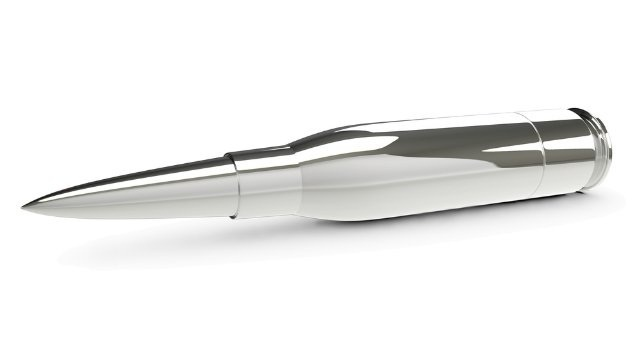
\includegraphics[width=11cm]{34d48c3.jpg}}
\frame[plain]{
\vspace{4cm}
\begin{center}
 {\LARGE \textcolor{color_titulo}{{\em No Silver Bullet}}}\\
 \vspace{.25cm}
 {\large Presentaci\'on de papers fundacionales -- Grupo $5$}\\
 \vspace{.5cm}
 {\bf {Ingenier\'ia del Software $2$}}\\
 \vspace{.5cm}
 {\small
    Facultad de Ciencias Exactas y Naturales\\
    Universidad de Buenos Aires \\
    $17$ de noviembre de $2014$ }
\end{center}
}
}

\begin{frame}[fragile]
  \frametitle{Qui\'en es \textit{Frederick P. Brooks, Jr.}}
\end{frame}

\begin{frame}[fragile]
  \frametitle{Introducci\'on}
\end{frame}


\begin{frame}[fragile]
  \frametitle{Dificultades esenciales}

  A diferencia del mundo del \textit{hardware} no podemos esperar que nuestra
  capacidad de producir buen \textit{sofware} se doble cada a\~no.

  De hecho, deber\'iamos considerar el caso del \textit{hardware} como una
  excepci\'on.

  La esencia de una entidad de \textit{software} es el resultado de la
  composici\'on no trivial de varios conceptos:
  \begin{itemize}
    \item conjuntos de datos
    \item relaciones entre datos
    \item algoritmos
    \item invocaci\'on de funciones
  \end{itemize}

  La parte dif\'icil de construir \textit{software} es la
  \textbf{especificaci\'on}, \textbf{dise\~no} y \textbf{testeo} de estos
  conceptos.
  La dificultad \textbf{no se encuentra} en la representaci\'on y el testeo
  de la fidelidad de la representaci\'on.

  \textbf{Los errores sint\'acticos son muy menores en comparaci\'on a los
  errores conceptuales en la mayor\'ia de los sistemas.}
\end{frame}


\begin{frame}[fragile]
  \frametitle{Complejidad}

  Las entidades de \textit{software} son complejas porque dos partes en un
  \textit{software} nunca son semejantes, si as\'i lo fuera, uno deber\'ia
  abstraerlas en una misma subrutina. Por este motivo el \textit{software}
  se diferencia de las computadoras, los edificios o los autom\'obiles, donde
  los elementos repetidos abundan.

  Lograr que una entidad de \textit{software} escale es complejo, pues los
  elementos interactuan de forma no lineal.

  La complejidad del \textit{software} es esencial, no accidental. Por lo tanto
  descripciones que abstraigan esta complejidad suelen abstraer la esencia.

  La complejidad genera:
  \begin{itemize}
    \item dificultad en la comunicaci\'on de un equipo
      $\mapsto$ fallas, costo, atraso del proyecto
    \item dificultad en la enumeraci\'on de los estados de un programa
      $\mapsto$ baja confiabilidad en el programa
    \item complejidad en las funciones 
      $\mapsto$ dificultad en el uso de las mismas
    \item complejidad en las estructuras usadas
      $\mapsto$ dificultades en la modificabilidad, problemas de seguridad
  \end{itemize}

\end{frame}


\begin{frame}[fragile]
  \frametitle{\textit{Conformity} (adaptaci\'on)}

  La f\'isica, y otras disciplinas, deben lidiar con objetos complejos, pero
  se basan en la expectativa de encontrar teor\'ias unificadas.
  Esta expectativa no conforta a la ingenier\'ia del \textit{software}.

  La complejidad con la que se encuentra una entidad de \textit{software}
  es arbitraria, generada por las muchas instituciones humanas y sistemas
  a los cuales, sus interfaces, deben acatar.

  En los (muchos) casos en que una entidad de \textit{software} debe adaptarse
  a otras interfaces, la complejidad que esto genera no puede ser simplificada
  por ning\'un redise\~no que incluya \'unicamente a dicha entidad.
\end{frame}


\begin{frame}[fragile]
  \frametitle{Modificabilidad}
  A diferencia de los objetos manufacturados \textit{f\'isicamente} (edificios,
  autom\'obiles o computadoras), las entidades de \textit{software} continuamente
  est\'an siendo forzadas a cambiar.

  Los motivos principales son dos:
  \begin{itemize}
    \item la funcionalidad de un sistema suele necesitar extenderse o modificarse
    \item a diferencia de objetos f\'isicamente concretos, el \textit{software}
      es infinitamente modificable
  \end{itemize}

  Un sistema exitoso sufrir\'a modificaciones. Mientras se lo encuentre \'util,
  los usuarios lo utilizar\'an en escenarios no contemplados, en otros dominios.
  M\'as a\'un, un sistema exitoso sobrevivir\'a a las maquinas para las cuales
  fue inicialmente construido, que, sabemos, cambian continuamente.
\end{frame}


\begin{frame}[fragile]
  \frametitle{Invisibilidad}
  El \textit{software} es invisibile, \textit{invisualizable}.
  Las abstracciones geom\'etricas suelen resaltar inconsistencias, pero
  la realidad del \textit{software} no est\'a naturalmente embebida
  en un espacio.

  Las herramientas m\'as comunes para la visualizaci\'on suelen ser poco claras,
  pues vemos demasiadas conexiones. Suele ser buena pr\'actica limitar los
  \textit{links} y preferir los grafos \textbf{jer\'arquicos}.

  La visualizaci\'on geom\'etrica es una de las herramientas conceptuales m\'as
  importantes de la mente humana. La dificultad de visualizar el \textit{software}
  no solo limita el dise\~no de una mente, \textbf{limita la comunicaci\'on entre
  varias mentes}.
\end{frame}


\begin{frame}[fragile]
  \frametitle{Dificultades accidentales que fueron resueltas}

  \begin{itemize}
    \item[Lenguajes de alto nivel]
      Liberaron a los programas de mucha de su complejidad accidental.
      Nuesta sofisticaci\'on en c\'omo pensar las estructuras de datos, los tipos
      de datos y las operaciones, se encuentra en crecimiento, pero es un crecimiento
      cada vez m\'as limitado.
    \item[Tiempo compartido]
      El efecto principal es la r\'apida respuesta de un sistema. A medida que
      tiende a cero, el \textit{delay} se torna imperceptible. Mas all\'a de
      este punto no pueden esperarse beneficios particularmente importantes.
    \item[Ambientes de programaci\'on unificados]
      Atacan a las dificultades accidentales de comunicar m\'ultiples programas.
  \end{itemize}
\end{frame}


\begin{frame}[fragile]
  \frametitle{Candidatos a \textit{silver bullet}}

  El lenguaje \textsc{Ada}.
  Esta secci\'on qued\'o un poco desactualizada, dada la enorme cantidad de
  lenguajes de alto nivel, especializados en resolver gran parte de los
  problemas accidentales con que se encuentra un programador.

  TODO: leer un poco sobre Ada.
\end{frame}


\begin{frame}[fragile]
  \frametitle{Programaci\'on orientada a objetos}
  Separamos dos conceptos ortogonales que llevan el mismo nombre.
  \begin{itemize}
    \item[Tipos abstractos de datos] El tipo de un objeto debe ser
      definido por un nombre, un conjunto de valores propios, y un conjunto
      de operaciones propias. \textbf{No} por su estructura interna.
    \item[Tipos jer\'arquicos] Permiten la definici\'on de interfaces generales
      que se pueden ir refinando, siempre que se lo necesite.
  \end{itemize}

  Dada su ortogonalidad pueden ser usados independientemente.
  Permiten evitar las dificultades accidentales de la implementaci\'on de un
  dise\~no, pero \textbf{la complejidad del dise\~no sigue siendo esencial}.
\end{frame}


\begin{frame}[fragile]
  \frametitle{Inteligencia artificial}
  Si bien muchas personas creen que la inteligencia artificial ser\'a la
  revoluci\'on que dar\'a mejoras de un orden de magnitud en productividad
  y calidad de \textit{software}, el autor no concuerda.

  Las t\'ecnicas utilizadas para reconocimiento de voz parecen tener muy
  poco que ver con las utilizadas en reconocimiento de im\'agenes y ambas
  parecen muy distintas de las utilizadas en sistemas expertos.
  Esto da la idea de que no se tienen t\'ecnicas generales para resolver
  problemas de \textit{decisi\'on}.
\end{frame}


\begin{frame}[fragile]
  \frametitle{Sistemas expertos}

  Un ejemplo interesante que se da es el un (potencial) sistema experto que
  funciona como asistente de testeo.
  A medida que se desarolla una aplicaci\'on, el sistema va adquiriendo reglas,
  pasando de sugerencias muy generales a sigerencias cada vez m\'as relacionadas
  con la estructura del sistema.

  El trabajo requerido para generar las reglas de diagn\'ostico es trabajo
  que deber\'a hacerse de todas formas. Si este es hecho de forma suficientemente
  general podr\'ia reducir la cantidad de trabajo a largo plazo.

  La contribuci\'on principal que puede dar un sistema experto es cuando se lo
  pone a servicio de programadores sin experiencia. Una herramienta que facilite
  y recomiende buenas pr\'acticas puede ser muy importante.
\end{frame}

\begin{frame}[fragile]
  \frametitle{Programaci\'on ``autom\'atica'' y programaci\'on gr\'afica}

  TODO
\end{frame}


\begin{frame}[fragile]
  \frametitle{Verificaci\'on de programas}
  TODO
\end{frame}

\begin{frame}[fragile]
  \frametitle{Ambientes de desarollo y \textit{hardware}}
  TODO
\end{frame}


\begin{frame}[fragile]
  \frametitle{Ataques prometedores contra la esencia conceptual}
  Comprar \textit{vs.} construir
  TODO
\end{frame}


\begin{frame}[fragile]
  \frametitle{Refinamiento de requerimientos y prototipado r\'apido}
  TODO
\end{frame}


\begin{frame}[fragile]
  \frametitle{Desarrollo incremental -- \textit{grow vs. build}}
  TODO
\end{frame}

\begin{frame}[fragile]
  \frametitle{Grandes dise\~nadores}
  TODO
\end{frame}

\begin{frame}[fragile]
  \frametitle{Conclusiones -- moraleja}
  TODO
\end{frame}
\end{document}
